
%%%%%%%%%%%%%%%%%%%%%%%%%%%%%%%%%%%%%%%%%%%%%%%%%%%%%%%%%%%%%%%%%%%%%%%%%%%%%%%%%%%%%%%%%%%%%%%%%%%%%%%%%%%%%%%


\begin{figure}
        \begin{minipage}[b]{0.45\linewidth}
            \centering
            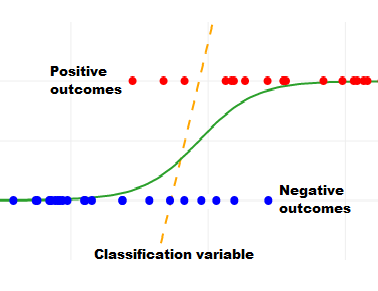
\includegraphics[width=\textwidth]{Figs/Classification/LogisticReg_5.png}
            % \caption{Predictive value of variables \\ (relation of score to positives and negatives)}
            \caption{Predictive value of classification variables}
        \end{minipage}
        \hspace{0.5cm}
        \begin{minipage}[b]{0.45\linewidth}
            \centering
            \includegraphics[width=\textwidth]{Figs/Classification/ROC_distns_1.png}
            % \caption{Difference in distributions of variables \\ (positives vs. negatives)}
            \caption{Difference in the distributions of variables}
        \end{minipage}
    % 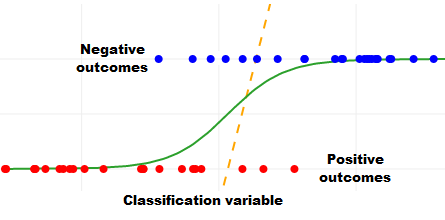
\includegraphics[scale =  0.5 ]{Figs/LogisticReg_3.png}%
    % \includegraphics[scale =  0.5 ]{Figs/ROC_distns_1.png}
\end{figure}




%\begin{figure}[h!]
%
%\begin{center}
%
%    \caption{Equivalence of Classification Models} \label{fig:classification1}
%
%    \begin{tabular}{c}
%
%        \subfloat[Classification Model]{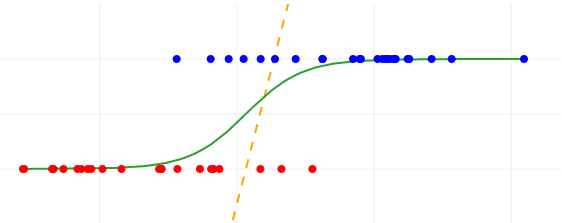
\includegraphics[scale=  0.50]{Figs/Classification/LogisticReg2.png}} \\
%
%
%        \subfloat[Difference of Distributions]{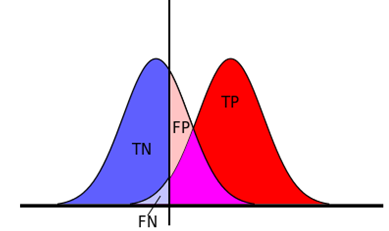
\includegraphics[scale=  0.50]{Figs/Classification/ClassModelDistns1.png}} \\
%
%
%
%
%    \end{tabular}
%
%\end{center}
%
%    \footnotesize
%
%        \textbf{Equivalence of Classification Models: }
%        Description goes here.
%
%\end{figure}


%%%%%%%%%%%%%%%%%%%%%%%%%%%%%%%%%%%%%%%%%%%%%%%%%%%%%%%%%%%%%%%%%%%%%%%%%%%%%%%%%%%%%%%%%%%%%%%%%%%%%%%%%%%%%%%

